\section{I2C - TWI}
Inter Integrated Circuit è un protocollo di comunicazione tra circuiti integrati inventato dalla Philips (ora NXP) per far comunicare i suoi circuiti integrati.
Essendo un nome registrato dalla Philips stessa chiunque escluso loro voglia utilizzarlo lo riferisce tramite un altro nome: TWI (two-wire interface).

\subsection{Digressione sulle proprietà intellettuali}
\subsubsection{Brevetto}
Si possono brevettare gli oggetti fisici, le molecole e gli organismi viventi (per esempio le mele gialle, alcuni tipi di rose, ecc) a patto che siano utili e che questi elementi non siano ovvi.
I brevetti devono essere pubblicati e solo chi lo depone ha il permesso di produrre l' elemento sotto brevetto, tutti gli altri possono guardare il brevetto ed eventualmente migliorarlo.
L' alternativa a questa pratica è il segreto industriale, usato ad esempio dalla Coca Cola.

Il brevetto scade dopo 15 anni e diventa libero per tutti.

\subsubsection{Registrazione del nome}
Si possono registrare i nomi associati alle tecnologie in modo da avere l' esclusiva sull' utilizzo.
E' proprio ciò che ha fatto la Philips con I2C quindi tutti possono implementare l' hardware che c'è alla base ma non possono usare pubblicamente il nome I2C.

La registrazione di un nome ha durata eterna finché la produzione dell' oggetto prosegue, dopo due anni dalla fine della produzione la registrazione decade e torna disponibile per la registrazione.
Si possono inoltre registrare diversi prodotti con lo stesso nome a patto che non possano essere scambiati:
per esempio posso registrare una marca di motoseghe e chiamarla nutella perché è impossibile confonderla con la crema spalmabile.

\subsubsection{Copyright}
E' una regisrazione di proprietà intellettuale che vale per 95 anni ed è applicabile a film, libri e canzoni.
Ci sono diverse regole sul copyright che danno lavoro ad avvocati specializzati.
Per esempio la matematica non può essere brevettata ma gli algoritmi sì (negli USA).

\subsection{Hardware}
I2C è un protocollo pensato per la comunicazione con tanti device, si tratta di un bus di comunicazione sviluppato su due fili (più la massa).
Nei calcolatori si usa per connettere i sensori ed eseguire letture.

\subsubsection{Gestione delle collisioni}
Essendo un bus è necessaria la gestione delle collisioni, in questo protocollo è implementata direttamente in hardware per evitare problemi software.
Si utilizza una configurazione ad open-drain (open-collector se si utilizzano i BJT) quindi i bus sono connessi a VCC attraverso dei resistori e i device apposti sul bus possono solo connettere il bus a GND.
Così facendo anche se due dispositivi comunicano allo stesso tempo non c'è possibilità di creare un cortocircuito:
\begin{figure}[H]
    \centering
    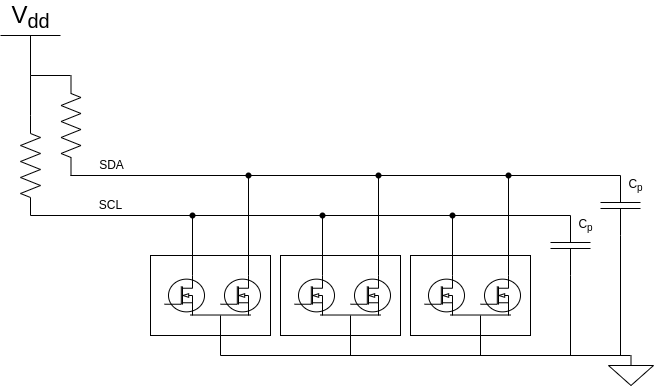
\includegraphics[width=300px]{images/24_I2C-TWI/i2c_bus.png}
\end{figure}
Si noti che per costruzione il bus ha una capacità parassita che chiameremo $C_p$, i resistori vanno scelti in modo che $\frac{1}{RC2\pi}$ sia maggiore di 400KHz, tuttavia $C_p$ non è nota perché dipende dalla geometria del filo utilizzato.

Il bus può arrivare fino a 10Mbit ma serve una costante di tempo molto piccola per arrivarci.

In genere un master parla ed uno slave ascolta mentre gli altri non fanno niente, se due trasmettessero allo stesso momento sulla linea ci sarebbe uno zero se almeno uno dei due è acceso, si tratta infatti di una wired-and, quindi se due dispositivi parlano allo stesso momento sul bus esso trasporta un segnale che è l' AND dei due segnali trasmessi.

\subsection{Protocollo}
I due fili utilizzati sono:
\begin{itemize}
    \item SDA: utilizzato per trasmettere i dati
    \item SCL: utilizzato per trasmettere il clock
\end{itemize}

Ogni dispositivo è identificato da un indirizzo a 7 bit di solito già impresso internamente nel chip stesso ed utilizzato anche come identificativo del tipo di componente.
Se infatti volessi avere più sensori dello stesso tipo, e quindi con identificatore uguale in genere il produttore mette a disposizione alcuni pin del chip per modificare i bit meno significativi dell' indirizzo.

I microcontrollori che di solito fanno da master invece hanno un apposito registro utilizzato per mantenere un ID scelto dal programmatore in modo da lasciare più libertà possibile.

L' indirizzo 0 è riservato ed utilizzato per altri scopi che vedremo in seguito.

NB: 7 bit di indirizzo sono successivamente risultati pochi quindi esiste un seguito dello standard che fa uso di indirizzi a 10 bit.

\subsubsection{Segnale di start}
In idle i due canali sono a livello alto grazie ai resistori di pull-up, quando un master inizia una transazione abbassa prima SDA e successivamente SCL:
\begin{figure}[H]
    \centering
    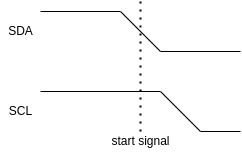
\includegraphics[width=150px]{images/24_I2C-TWI/i2c_start_signal.png}
\end{figure}

\subsubsection{Segnale di stop}
Quando la transazione sta finendo o quando deve essere abortita a causa di un qualsiasi problema si deve alzare prima SCl e successivamente SDA:
\begin{figure}[H]
    \centering
    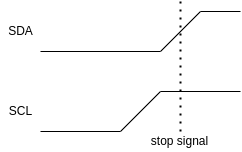
\includegraphics[width=150px]{images/24_I2C-TWI/i2c_stop_signal.png}
\end{figure}
Il segnale di stop causa su tutti i ricevitori un reset.

\subsubsection{Comunicazione}
Una comunicazione si compone di:
\begin{itemize}
    \item segnale di start
    \item indirizzo a 7 bit dello slave inviato in big endian
    \item ottavo bit utilizzato per specificare l' operazione:
    \begin{itemize}
        \item 1 per leggere
        \item 0 per scrivere
    \end{itemize}
    \item ACK o NACK da parte dello slave per dire che ha capito o non ha capito.
    Se non c'è nessuno a quell' indirizzo il master se ne accorge e la comunicazione finisce
\end{itemize}

\begin{figure}[H]
    \centering
    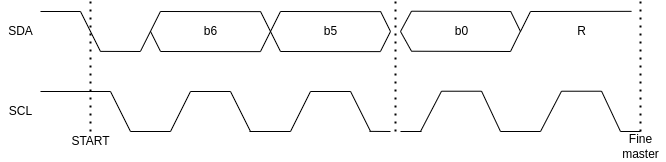
\includegraphics[width=330px]{images/24_I2C-TWI/i2c_address_transmission.png}
\end{figure}

Tutti gli slave ascoltano da quando notano un segnale di start e smettono di ascoltare appena si accorgono che l' indirizzo richiesto non è il proprio.

Dopo gli 8 bit inviati il clock viene mantenuto basso ed il master smette di pilotare SDA.
Lo slave inizia a pilotare SDA:
\begin{itemize}
    \item se tiene alta la linea è un NACK (può anche essere assenza di slave in quanto la linea di default è alta)
    \item se abbassa la linea è un ACK
\end{itemize}

Al 9° impulso di clock il master ha capito e se ha ricevuto un ACK continua a pilotare SCL per sincronizzare lo slave e permettergli di scrivere i dati se si è richiesta una lettura.
Se invece si è richiesta una scrittura dopo l' ACK il master invia i dati, dopodiché si aspetta l' ACK dello slave sui dati.
In successione si possono inviare uno stop bit oppure altri byte di dati.

\begin{figure}[H]
    \centering
    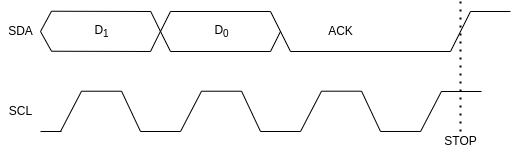
\includegraphics[width=250px]{images/24_I2C-TWI/i2c_ack_stop.png}
\end{figure}

\subsection{Esempio con una RAM I2C}
\subsubsection{Scrittura}
Supponiamo di voler scrivere su una RAM I2C:
\begin{itemize}
    \item inviamo l' indirizzo del dispositivo
    \item inviamo il bit di scrittura
    \item aspettiamo l' ACK
    \item inviamo il codice operativo della operazione da eseguire
    \item inviamo 4 byte di indirizzo al quale si vuole scrivere
    \item inviamo i dati da scrivere
\end{itemize}

\subsubsection{Lettura}
Dal momento che dobbiamo inviare il codice operativo e l' indirizzo della locazione di memoria da leggere ma poi dobbiamo anche lasciare spazio allo slave di scriverci i dati memorizzati dovremmo poter invertire la direzione di trasmissione, cosa che non si può fare con lo standard che abbiamo visto fino ad ora.
Potremmo pensare di eseguire tutto in due transazioni ma alla fine della prima si deve inviare uno stop bit che causa il reset dei dispositivi slave.

\subsection{Repeated start}
Per sopperire alla mancanza di un meccanismo per modificare la direzione dei dati esiste il repeated start, dopo l' indirizzo, il comando ed altri eventuali dati si può inserire un secondo start bit con un secondo comando.

Nel caso della RAM I2C dopo aver inviato il comando di lettura dalla RAM e l' indirizzo al quale leggere si inserisce il repeated start con il comando lettura ed in questo momento la RAM inizia a trasmettere  i dati che ha memorizzato:
\begin{figure}[H]
    \centering
    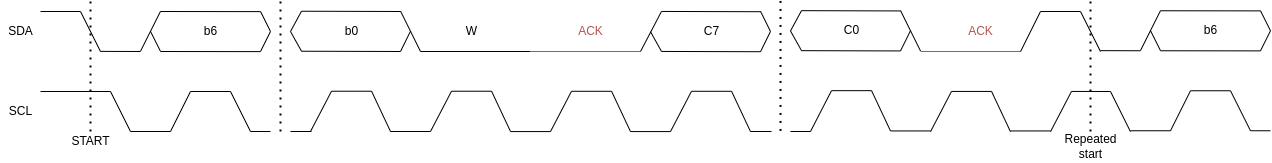
\includegraphics[width=330px]{images/24_I2C-TWI/i2c_repeated_start.png}
\end{figure}

\subsection{Collisioni tra master}
Se due master inviano uno start bit allo stesso tempo (quindi iniziano la comunicazione), se fanno lo stesso indirizzo sulla linea c'è l' AND delle linee e quindi nessuno si accorge di niente, se invece trasmettono dati diversi chi fa l' 1 si accorge della collisione e smette (si dice che perde l' arbitraggio).
Dato che l' indirizzo viene trasmesso in big endian la collisione è vinta da chi contatta l' indirizzo più basso.
A parità di indirizzo invece vince chi scrive (quindi chi pone lo 0 sulla linea).

\subsection{Gestione del flusso}
Uno slave può obbligare il master a rallentare in caso esso trasmetta un clock troppo veloce, per fare ciò quando il master tiene a 0 il clock lo fa anche lo slave, quando il master pone 1 allora lo slave continua a tenere 0 finché non è pronto ad andare avanti.
Di questo comportamento il master se ne accorge e quindi rallenta aspettando lo slave.

\subsection{Registri}
\subsubsection{TWBR}
Contiene il prescaler del generatore di clock.

\subsubsection{TWCR}
\begin{figure}[H]
    \centering
    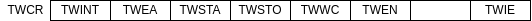
\includegraphics[width=320px]{images/24_I2C-TWI/TWCR.png}
\end{figure}
\begin{itemize}
    \item TWINT: è il flag relativo all' interruzione causato dalla terminazione di una transazione. Va resettato a mano alla fine dell' handler scrivendovi 1 sopra.
    Una volta ripulito il flag parte una transazione su TWI
    
    \item TWEA: abilita la risposta con acknowledge se un master ci contatta
    
    \item TWSTA: scrivendo su questo bit si causa l' inserimento di uno start bit sulla linea se è libera
    
    \item TWSTO: scrivendo su questo bit si causa l' inserimento di uno stop bit sulla linea
    
    \item TWWC: settato quando si sta facendo un uso sbagliato della periferica, come ad esempio scrivere su TWI e TWDR mentre TWINT è basso
    
    \item TWEN: abilita la periferica
    
    \item TWIE: abilita le interruzioni
\end{itemize}

\subsubsection{TWSR}
\begin{figure}[H]
    \centering
    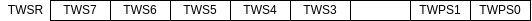
\includegraphics[width=320px]{images/24_I2C-TWI/TWSR.png}
\end{figure}
\begin{itemize}
    \item TWPS0-1: prescaler del bit rate
    \item TWS7-3: indicano lo stato della periferica
\end{itemize}

\subsubsection{TWDR}
Contiene il prossimo dato da inviare se in modalità trasmissione o l' ultimo byte letto se in modalità ricezione.

\subsubsection{TWAR}
\begin{figure}[H]
    \centering
    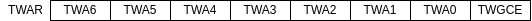
\includegraphics[width=320px]{images/24_I2C-TWI/TWAR.png}
\end{figure}
\begin{itemize}
    \item TWA6-0: bit usati per impostare l' indirizzo del uC
    \item TWGCE: indica se il uC deve rispondere alla chiamata sull' indirizzo 0
\end{itemize}


